\documentclass[11pt, a4paper]{article}

% ----- Packages -----
\usepackage[utf8]{inputenc}
\usepackage{amsmath, amssymb}
\usepackage{geometry}
\geometry{top=1in, bottom=1in, left=1in, right=1in}
\usepackage{float}
\usepackage{tikz}
\usetikzlibrary{arrows.meta, positioning, calc}

% ----- Advanced TikZ Styles -----
\tikzset{
    feNode/.style={
        circle, 
        draw=black, 
        fill=white, 
        thick, 
        inner sep=0pt, 
        minimum size=1.8mm
    },
    feLine/.style={
        line width=1.5pt
    },
    dimLine/.style={
        {Latex[length=2.5mm, width=1.5mm]}-{Latex[length=2.5mm, width=1.5mm]}, 
        thin
    },
    extLine/.style={
        thin, 
        draw=black!70
    }
}

\begin{document}

% ----- Header -----
\begin{center}
    {\Large \textbf{Homework 2}} \\[0.2cm]
    {\large \textbf{CE 512 Finite Element Method}} \\[0.1cm]
    {\large 2026 Spring} \\[0.3cm]
    \textbf{Due Date:} 09.03.2026-01:00 (upload to \texttt{https://cloud-lms.iyte.edu.tr})
\end{center}

\vspace{0.5cm}

% ----- Introduction -----
\noindent The following figure shows a 4 element truss structure. All elements have the same cross section and modulus of elasticity. Use hand calculations to solve the following questions.

\vspace{0.2cm}

\begin{enumerate}
    \item[a)] Construct the global stiffness matrix of the structure
    \item[b)] Compute the nodal displacements,
    \item[c)] Compute the strains in each element,
    \item[d)] Suppose the force P increases until the first member yields. Which member yields first and what is the value of P?
    \item[e)] Now consider the case at which the force P increases until the first member buckles. Which member buckles first, and what is the value of P?
\end{enumerate}

\vspace{0.3cm}
\noindent Let $E=20~000$ MPa and $\sigma_{y}=300$ MPa. The member cross section is a square hollow section with outer dimensions $40~\text{mm}\times40~\text{mm}$ and thickness $2.5~\text{mm}$.
\vspace{0.5cm}

% ----- Diagram -----
\begin{figure}[H]
    \centering
    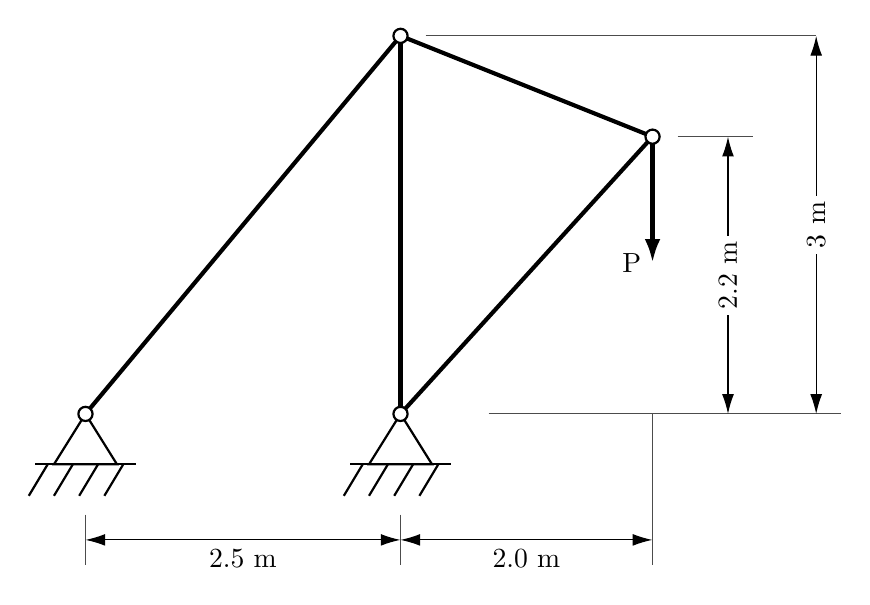
\begin{tikzpicture}[scale=1.6, >={Latex[length=3mm, width=2mm]}]
        
        % Coordinate Definitions
        \coordinate (N1) at (0, 0);       % Bottom Left
        \coordinate (N2) at (2.5, 0);     % Bottom Middle
        \coordinate (N3) at (2.5, 3.0);   % Top
        \coordinate (N4) at (4.5, 2.2);   % Right
        
        % Element Lines
        \draw[feLine] (N1) -- (N3);
        \draw[feLine] (N2) -- (N3);
        \draw[feLine] (N2) -- (N4);
        \draw[feLine] (N3) -- (N4);
        
        % Macro for Pinned Support
        \def\drawPinSupport#1{
            \draw[thick] (#1) -- ++(-0.25, -0.4) -- ++(0.5, 0) -- cycle;
            \draw[thick] (#1) ++(-0.4, -0.4) -- ++(0.8, 0);
            \foreach \i in {-0.3, -0.1, 0.1, 0.3} {
                \draw[thick] (#1) ++(\i, -0.4) -- ++(-0.15, -0.25);
            }
        }
        
        % Draw Supports
        \drawPinSupport{N1}
        \drawPinSupport{N2}
        
        % Applied Force P (Çizim sırası öne alındı ki node'un altında kalsın)
        % P harfi okun ucuna (pos=1) ve soluna (left) alındı
        \draw[->, line width=1.5pt] (N4) -- ++(0, -1.0) node[pos=1, left] {P};
        
        % Nodes (Çizgilerin ve okların üstünde kalması için en son çizdiriliyor)
        \node[feNode] at (N1) {};
        \node[feNode] at (N2) {};
        \node[feNode] at (N3) {};
        \node[feNode] at (N4) {};
        
        % ---------------------------------------------------------
        % Dimensioning
        % ---------------------------------------------------------
        
        % Horizontal Extension Lines
        \draw[extLine] (N1) ++(0, -0.8) -- ++(0, -0.4);
        \draw[extLine] (N2) ++(0, -0.8) -- ++(0, -0.4);
        \draw[extLine] (N4) ++(0, -2.2) -- ++(0, -1.2); % Drops from N4 to base
        
        % Horizontal Dimension Lines & Text
        \draw[dimLine] (0, -1.0) -- (2.5, -1.0) node[midway, below] {$2.5$ m};
        \draw[dimLine] (2.5, -1.0) -- (4.5, -1.0) node[midway, below] {$2.0$ m};
        
        % Vertical Extension Lines
        \draw[extLine] (3.2, 0) -- (6.0, 0); % Bottom reference baseline extending right
        \draw[extLine] (N4) ++(0.2, 0) -- ++(0.6, 0);
        \draw[extLine] (N3) ++(0.2, 0) -- ++(3.1, 0);
        
        % Vertical Dimension Lines & Text
        \draw[dimLine] (5.1, 0) -- (5.1, 2.2) node[midway, fill=white, inner sep=2pt, rotate=90] {$2.2$ m};
        \draw[dimLine] (5.8, 0) -- (5.8, 3.0) node[midway, fill=white, inner sep=2pt, rotate=90] {$3$ m};
        
    \end{tikzpicture}
    \caption{Truss structure}
\end{figure}

\end{document}
